\chapter{TMTO-Attack}

\label{ch:tmto}

\newpage
\section{Hellman Tables}
Hellman tradeoff is the first iteration of time memory trade offs, It was first explained in the paper A Cryptanalytic Time - Memory Trade-Off by Martin Hellman.
The idea is similar to a naive table lookup where all possible keys K have been encrypted with the plaintext P. Instead of storing all the key ciphertext pairs which is done in the naive table lookup all pairs are sorted into several chains where the only part stored is the start point and the end point. This way memory is saved but time is increased for the online phase. To find a pair one needs to find the right chain and look up the pair.


\subsection*{Precomputation phase}
Like any other tmto the table itself is generated in the precomputational phase.Each table is fixed for a single plaintext. The plaintext is encrypted with the selected encryption function E, the key is a arbitarily selected from all possible N keys. This results in the ciphertext C which is in turn used as the next key for the next encryption of the plaintext. A reduction function is applied to C which has the purpose to reduce the bit length of C and re-randomize the output.

The Helman tradof has 3 main parameters, m, t and l and they decide the size of the table that will be generated.
m is the amount of rows, t is the columns, and l is the amount of times they are repeated.
Certain requirements are put on these parameters, The size of m*t*t must not be much larger or much smaller than N.
N is the keysize of the cipher we are trying to break. We use a Matrix stopping constant (Hmsc) to hold the difference between N and m*t*t. Hmsc can therefore not be very large nor very close to zero.

add om reduction function

By selecting the parameters the table can be generated. This is done by selecting m random starting points, $ sp^{k}_1,sp^{k}_2,...,sp^{k}_m E N$. Each startingpoint is then used as the start of their chain and with recursion the chain links are computed by $ x^{k}_{i,j}=F_k( x^{k}_{i,j-1})$ for $0<j<=t$. When the endpoint is reached it is stored as a pair with the startpoint ${( sp^{k}_{i}, ep^{k}_{i})}^{m}_{i=1}$.
The Hellman table/matrix is usually visualized like so:
\\
\begin{figure}[t]
  figure from Making better tmto paper
  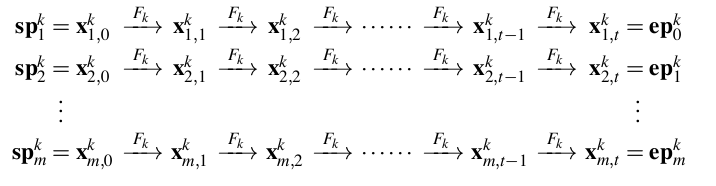
\includegraphics[width=\textwidth]{figures/HellmanMatrix.png}
  \centering
\end{figure}

Here the starting points are sp they are equal to x which is the first element of the chain. It is then encrypted with the current encryption scheme and the reduction function is applied. This is doen t times and $e_t$ is the endpoint.

insert drawing of how Helman chain works
Each row/chain from figure 1 is built the way shown in figure2. E is the encryption K is the key SP start point R reduction function and X is the ciphertext for each chain link. When a table is generated it should contain m touples of (SP,EP) and every chain should contain t+1 keys which results in m x (t+1) keys. This should mean that our tables coverage should be m x t, this is not always the case due to merges.
There are m $x$ t different chain links and it can happen that some of them merge.


\subsubsection{Merges}
Merges happen when in some point of the generation two chains have the same chain link there is a collision and the chains merge. This can be caused by the reduction function, if the reduction function reduces the size of bits of the Ciphertext. If we have ciphertext1 12345678 and ciphertext2 12345679 we have 32 bits here but our encryption only takes 28 bits then this would be a merge if the reduction function just removes the last 4 bit. The chains have now merged and the following intermediate points(chains) will now be the same. This affects coverage, if the merge happens 10 steps into the chain the coverage  will have 10 - t less keys since the two chains will be duplicate.

illustration of merges
\subsubsection{Loops}
Loops occur when a intermediete point(chain link) points back to a previously reached chain link. This also decreases the tables coverage.

figur for chain looping

A loop will loop around in the same chain links untill it reaches t.

\subsubsection {Multiple Tables}
In Hellman as m and t increases it will reach a point where the coverage doesnt increase due to merges and loops. This has been calculated to be somewhere near $N^{\frac{2}{3}}$ for single tables. This is the reason that the upper bounds for M and T are around $N^\frac{1}{3}$

\subsection*{Online phase}
Once a table is generated and we have a matching text ciphertext pair (y=F(x)) the online phase can commence.\\
The given ciphertext is used as the key for the encryption and we compute a single chain. This is done the same way as shown in figure 2 each link computed is matched with the computed Hellman table. This is done for all indicies l in the table if a match isnt found the algorithm will report faliure.\\

Whenever a match is found the corresponding SP is returned. The chain is now partially regenerated to obtain $X_{tmp}=x^k_{i,t-j}=F^{t-j}_k(sp^k_i)$. Which should be the key the text was encrypted with:
\begin{equation}
    F^j_k(x_{tmp})=F^j_k(F^(t-j)_k(sp^k_i))=ep^k_i=y^k_j=F^{j-1}_k(y_1)=F^j_k(x)
\end{equation}
\subsubsection{False Alarms}
False alarms happen when in the onlinephase a match is found, but the chain did not contain a valid key. This can happen when a merge has happend earlier when two different chains point to the same end point.
\\
Skal mere paa her
\subsection*{Analysis}
This section will address the success probability, cost of resolving alarms, tradeofcurve, memory Usage, precomputational time and online time.


\subsubsection*{Success probability}
The success probability of the table is found by calculalting how many keys that are covered in our table. Increasing the size of the table will increase the probability that the key is in it. The amount of keys that are covered depends on the amount of startpoints and the size of each chain. The success ratio of a single table can be calculated the following way:
Lower bound from hellman paper
$\frac{|HM|}{N}>=\frac{1}{N}\sum^{t}_{j=1}\sum^{m}_{i=1}(1-\frac{it}{N})^{j} $
When the all the tables are prcessed and assuming the reduction functions provide independent results the success probability becomes:
\[1-(1-\frac{|HM|}{N})^l\approx 1- exp(-\frac{l|HM|}{N})\]
Since the count of duplicates is maintained by the matrix stopping rule, the size of the table is :$|HM|\approx mt$.
\subsubsection{Cost of resolving alarms}
The amount of false alarms a table receive is given by $\frac{H_{msc}}{2}$\cite{14 in 176}, which leads to the cost of resolving them. The cost of resolving alarms are the following:
\begin{equation}
\text{(cost of resolving alarms for all tables)}>=\frac{H_{msc}}{6}lt
\end{equation}
proof found in \cite{18 in 176}
\begin{equation}
\text{(expected cost of resolving alarms)}=\frac{H_{msc}}{6}t
\end{equation}
proof found in \cite{15 in 176}
\subsubsection{Tradeofcurve}
The tradeoff curve is
\subsubsection{Memory Usage}
\subsubsection{Precomputational time}
\subsubsection{Online time}

\section{Distinguished Points Tables}
The distinguished points - tradeof was first described by Rivest in
the book [ref]. It is a simple modification of the Hellman tradeoff
where one does not have chains of the same size, since when a
distinguished point is reached the chain does not continue. The way we distinguish any point from a dp by some property (eg. the first 16 bits are zero). This is the DP proporty, with DP-tradeoff the amount of table lookups is lowered dramatically since the only lookups happen when a point with a DP property is found.
\subsection{Precomputational phase}
The online phase of the DP-tradeoff is very similar to the Hellman method.
\subsubsection{Parameters}
There are several parameters that decide the size and the coverage of
the DP-tradeoff. M is the amount of rows, t is the chain length  and l is the amount of tables.
To prevent chains from growing uncontrollably $t_{max}$ is used. This is the max size a chain can get before it is aborted and the chain discarded.
Like the Hellman tradeoff the table must satisfy the
given matrix stopping rule $mt^2\approx N$ again the difference between
mt and N should not be too large or to close to zero. Again a
matrixstopping constant is used to hold the difference $mt^2\approx
D_{msc}N$. Reduction functions are selected.... add more. The dp property is given by a bitmask with length $dp_l$.
Once the Parameters have been selected the algorithm can start. $F(SP)=C_1$ is computed and the reduction function is applied which gives the first chain link.$C_1$ is compared to the Dp property, if it is a positive match $C_1$ is an EP this is stored with the SP and the chain length $t_{DP}$. If $C_1$ does not match up with the dp property $F(C_1)=C_2$ is computed and the result compared to the dp property this is done untill an EP is found or the chain length reaches $t_max$


\begin{figure}[th]
  DP schema
  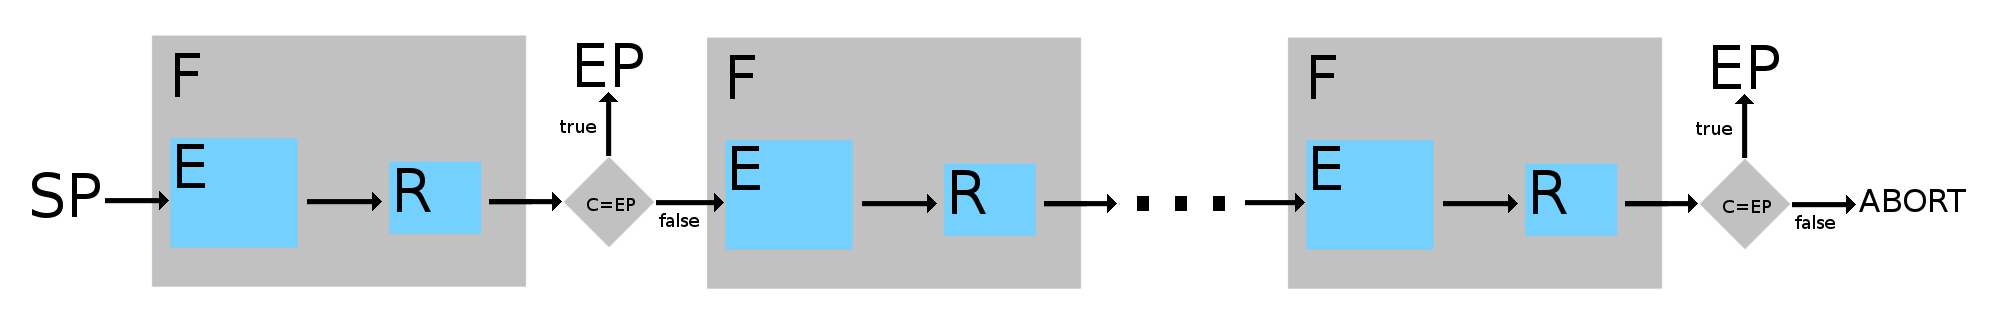
\includegraphics[width=\textwidth]{figures/DPSchema.png}
  \centering
\end{figure}

A DP table does not have duplicate keys, due to it's built in loop/merge detection. If a merge or a loop happens the table will select the chain that is the longest which in turn will result in more unique keys.
\subsubsection{Merges and Loops}
If two chains A and B have an identical chain link (intermediate point) $X_A = X_B$. If $X_A$ is reached in step n and $X_B$ is reached in k steps where $k>n$ holds then $X_B$ is stored and $X_A$ is discarded. This only holds when both chains reach an EP. Loops will never be stored in the table since it will never reach a point where the dp property holds and will therefore reach $t_{max}$ and be discarded.

\subsection{Online phase}
The online phase for the DP-tradeoff is also similar to the Hellman-tradeoff online phase. The major difference is that all EP in the computed table are distinguished points therefore instead of checking all chain links that the given ciphertext gives we only check it when a DP is reached. F is applied to C until a DP is reached or it has been applied $t_{max}-1$ times. If it reaches $t_{max}-1$ the key is not covered in the table but if it is reached we check the table for the distinguished point/EP when found we regenerate the chain from the stored SP, Just like in the Hellman tradeoff. When resolving false alarms we we either have to regenerate the entire chain untill the EP is reached or the $y^k_1$ (WHAT IS THIS). This can be prevented by storing the size of each chain in the table, this wil in turn cause the table to be larger.

\subsection{Analysis}
The size of the dp property directly influences the table, if the dp property is small(the first 4 byte are 0) then chains will be short since the probability of getting a point where the first 4 byte is 0 is bigger than if it was the first 5,7 or 10. This also holds when the dp property is too large this results in fewer matches on the dp property therefore longer chains. The property should satisfy by a random element of $N$ with probability $\frac{1}{t}$. The average length should then be t.

\subsubsection{Success Ratio}
The success ratio for the DP tradeoff
\subsubsection{}
\section{Rainbow Tables}
\label{sec:raintheory}
\subsection{Precomputation phase}
\subsection{Online phase}

%%% Local Variables:
%%% mode: latex
%%% TeX-master: "Thesis"
%%% End:
